\documentclass{beamer}
\usefonttheme[onlymath]{serif}
\usepackage[T1]{fontenc}
\usepackage[utf8]{inputenc}
\usepackage[english, icelandic]{babel}
\usepackage{amsmath}
\usepackage{amssymb}
\usepackage{amsthm}
\usepackage{gensymb}
\usepackage{parskip}
\usepackage{mathtools}
\usepackage{listings}
\usepackage{hyperref}
\usepackage{graphicx}
\usepackage{color}
\usepackage{enumerate}
\usepackage{tikz}
\usetikzlibrary{calc}
\usetikzlibrary{positioning}
\usetikzlibrary{angles}
\usetikzlibrary{shapes}
\usetikzlibrary{arrows}
\usepackage{verbatim}
\usepackage{multicol}
\usepackage{array}
\usepackage{minted}
\parskip 0pt

\usepackage{colortbl}
\usepackage{pgf}
\usepackage{pgfkeys}
\usetikzlibrary{fpu}
\usepackage{tkz-euclide}

\DeclareMathOperator{\lcm}{lcm}
\newcommand\floor[1]{\left\lfloor#1\right\rfloor}
\newcommand\ceil[1]{\left\lceil#1\right\rceil}
\newcommand\abs[1]{\left|#1\right|}
\newcommand\p[1]{\left(#1\right)}
\newcommand\sqp[1]{\left[#1\right]}
\newcommand\cp[1]{\left\{#1\right\}}
\newcommand\norm[1]{\left\lVert#1\right\rVert}
\renewcommand\Im{\operatorname{Im}}
\renewcommand\Re{\operatorname{Re}}

\usetheme{metropolis}
\definecolor{dark yellow}{rgb} {0.6,0.6,0.0}
\definecolor{dark green}{rgb} {0.0,0.6,0.0}

\graphicspath{{myndir/}}

\tikzstyle{vertex}=[circle,fill=black!50,minimum size=15pt,inner sep=0pt, font=\small]
\tikzstyle{selected vertex} = [vertex, fill=red!24]
\tikzstyle{edge} = [draw,thick,-]
\tikzstyle{dedge} = [draw,thick,->]
\tikzstyle{weight} = [font=\scriptsize,pos=0.5]
\tikzstyle{selected edge} = [draw,line width=2pt,-,red!50]
\tikzstyle{selected2 vertex} = [vertex, fill=hilight!50, text=black]
\tikzstyle{ignored edge} = [draw,line width=5pt,-,black!20]
\tikzstyle{vertex1} = [vertex, fill=red]
\tikzstyle{vertex2} = [vertex, fill=blue]
\tikzstyle{vertex3} = [vertex, fill=green, text=black]
\tikzstyle{vertex4} = [vertex, fill=yellow, text=black]
\tikzstyle{vertex5} = [vertex, fill=pink, text=black]
\tikzstyle{vertex6} = [vertex, fill=purple]

\tikzset{
  treenode/.style = {align=center, inner sep=0pt, text centered,
    font=\sffamily},
  vertex/.style = {treenode, circle, black, font=\sffamily\bfseries\tiny, draw=black, text width=1.8em},% arbre rouge noir, noeud noir
  rvertex/.style = {treenode, circle, black, font=\sffamily\bfseries\tiny, draw=red, text width=1.8em},% arbre rouge noir, noeud noir
}

\definecolor{offwhite}{RGB}{249,242,215}
\definecolor{foreground}{HTML}{23373b}
\definecolor{background}{RGB}{24,24,24}
\definecolor{title}{RGB}{107,174,214}
\definecolor{gray}{RGB}{155,155,155}
\definecolor{subtitle}{RGB}{102,255,204}
\definecolor{lolight}{RGB}{155,155,155}
\definecolor{green}{RGB}{125,250,125}

\definecolor{hilight}{RGB}{235,129,27}
\definecolor{vhilight}{HTML}{14B03D}

\def\hepta{\draw[foreground](A) -- (B) -- (C) -- (D) -- (E) -- (F) -- (G) -- cycle;}

\newcommand{\slice}[1]{%
    \hepta
    \draw[foreground] \foreach \x/\y in {#1} {(\x)--(\y)};
}

\title{Weighted Graphs}
\author{Arnar Bjarni Arnarson \and Atli FF}
\institute{\href{http://ru.is/td}{School of Computer Science} \\[2pt] \href{http://ru.is}{Reykjavík University}}
\titlegraphic{\hfill
\includegraphics[height=0.6cm]{../../shared/kattis}}

\begin{document}
\maketitle

\begin{frame}[plain]{Today we're going to cover}
    \begin{itemize}
        \item Topological sort
        \item Strongly connected components
        \item Minimum spanning tree
        \item Shortest paths
    \end{itemize}
\end{frame}

\begin{frame}[plain]{Topological sort}
    \vspace{5pt}
    \begin{itemize}
        \item We have $n$ tasks
        \item Each task $i$ has a list of tasks that must be completed before we can start task $i$
        \item Find an order in which we can process the tasks
        \vspace{5pt}
        \item Can be represented as a directed graph
            \begin{itemize}
                \item Each task is a vertex in the graph
                \item If task $j$ should be finished before task $i$, then we add a directed edge from vertex $i$ to vertex $j$
            \end{itemize}
        \vspace{5pt}
        \item Notice that this can't be solved if the graph contains a cycle
        \vspace{5pt}
        \item A modified depth-first search can be used to find an ordering in $O(n + m)$ time, or determine that one does not exist
    \end{itemize}
\end{frame}

\begin{frame}[plain,fragile]{Topological sort}
    \begin{minted}[fontsize=\scriptsize]{cpp}
vector<int> adj[1000];
vector<bool> visited(1000, false);
vector<int> order;

void topsort(int u) {
    if (visited[u]) {
        return;
    }

    visited[u] = true;
    for (int i = 0; i < adj[u].size(); i++) {
        int v = adj[u][i];
        topsort(v);
    }

    order.push_back(u);
}

for (int u = 0; u < n; u++) {
    topsort(u);
}
    \end{minted}
\end{frame}

\begin{frame}[plain]{Strongly connected components}
    \vspace{10pt}
    \begin{itemize}
        \item We know how to find connected components in undirected graphs
        \item But what about directed graphs?
        \vspace{10pt}
        \item Such components behave a bit differently in directed graphs, especially since if $v$ is reachable from $u$, it doesn't mean that $u$ is reachable from $v$
        \vspace{10pt}
        \item The definition remains the same, though
        \item A strongly connected component is a maximal subset of the vertices such that each pair of vertices is reachable from each other
    \end{itemize}
\end{frame}

\begin{frame}[plain]{Strongly connected components}
    \vspace{40pt}
    \begin{itemize}
        \item The connected components algorithm won't work here
        \vspace{10pt}
        \item Instead we can use the depth-first search tree of the graph to find these components
        \vspace{10pt}
        \item \textit{see example}
    \end{itemize}
\end{frame}

\begin{frame}[plain,fragile]{Strongly connected components}
    \begin{minted}[fontsize=\footnotesize]{cpp}
vector<int> adj[100];
vector<int> low(100), num(100, -1);
vector<bool> incomp(100, false);
int curnum = 0;

stack<int> comp;

void scc(int u) {

    // scc code...
}

for (int i = 0; i < n; i++) {
    if (num[i] == -1) {
        scc(i);
    }
}
    \end{minted}
\end{frame}

\begin{frame}[plain,fragile]{Strongly connected components}
    \begin{minted}[fontsize=\tiny]{cpp}
void scc(int u) {
    comp.push(u);
    incomp[u] = true;

    low[u] = num[u] = curnum++;
    for (int i = 0; i < adj[u].size(); i++) {
        int v = adj[u][i];
        if (num[v] == -1) {
            scc(v);
            low[u] = min(low[u], low[v]);
        } else if (incomp[v]) {
            low[u] = min(low[u], num[v]);
        }
    }

    if (num[u] == low[u]) {
        printf("comp: ");
        while (true) {
            int cur = comp.top();
            comp.pop();
            incomp[cur] = false;
            printf("%d, ", cur);
            if (cur == u) {
                break;
            }
        }

        printf("\n");
    }
}
    \end{minted}
\end{frame}

\begin{frame}[plain]{Strongly connected components}
    \vspace{30pt}
    \begin{itemize}
        \item Time complexity?
        \item Basically just the DFS analyze function (which was $O(n + m)$), with one additional loop to construct the component
        \item But each vertex is only in one component...
        \item Time complexity still just $O(n + m)$
    \end{itemize}
\end{frame}

\begin{frame}[plain]{Example problem: Tourist safety}
    Tourists sometimes like to explore the cities they're in. They start at
    their hotel, and then drive randomly around the city. This can be
    dangerous, however, as when the tourist becomes tired and wants to go home,
    it may not be possible!

    Given a directed road network, determine which road intersections are
    tourist-safe. A road intersection $u$ is tourist-safe if for each road
    intersection $v$ reachable from $u$, $u$ is reachable from $v$.
\end{frame}

\begin{frame}[plain]{Weighted graphs}
    \begin{itemize}
        \item Now the edges in our graphs may have weights, which could represent
            \begin{itemize}
                \item the distance of the road represented by the edge
                \item the cost of going over the edge
                \item some capacity of the edge
            \end{itemize}

        \item We can use a modified adjacency list to represent weighted graphs
    \end{itemize}
\end{frame}

\begin{frame}[plain,fragile]{Weighted graphs}
    \begin{columns}[T]
        \begin{column}{.4\textwidth}
            \begin{minted}[fontsize=\footnotesize]{cpp}
struct edge {
    int u, v;
    int weight;

    edge(int _u, int _v, int _w) {
        u = _u;
        v = _v;
        weight = _w;
    }
};
            \end{minted}
        \end{column}%
        \hfill%
        \begin{column}{.6\textwidth}
            \begin{figure}
                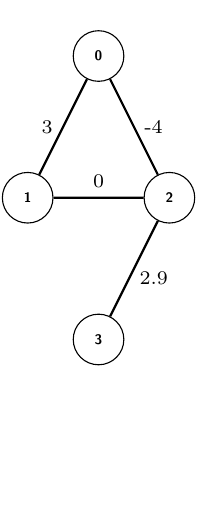
\begin{tikzpicture}[scale=1.8,auto,swap]
                    \node[vertex] (0) at (0.5,3) {0};
                    \node[vertex] (1) at (0,2) {1};
                    \node[vertex] (2) at (1,2) {2};
                    \node[vertex] (3) at (0.5,1) {3};

                    \path[edge] (0) -- node[weight,left] {3} (1);
                    \path[edge] (0) -- node[weight,right] {-4} (2);
                    \path[edge] (1) -- node[weight,above] {0} (2);
                    \path[edge] (2) -- node[weight,right,pos=0.6] {2.9} (3);

                    \pgfresetboundingbox
                    \path [use as bounding box] (0,0) rectangle (1,3.2);
                \end{tikzpicture}
            \end{figure}
        \end{column}%
    \end{columns}
\end{frame}

\begin{frame}[plain,fragile]{Weighted graphs}
    \begin{columns}[T]
        \begin{column}{.4\textwidth}
            \begin{minted}[fontsize=\footnotesize]{cpp}
vector<edge> adj[4];

adj[0].push_back(edge(0, 1, 3));
adj[0].push_back(edge(0, 2, -4));

adj[1].push_back(edge(1, 0, 3));
adj[1].push_back(edge(1, 2, 0));

adj[2].push_back(edge(2, 0, -4));
adj[2].push_back(edge(2, 1, 0));
adj[2].push_back(edge(2, 3, 2.9));

adj[3].push_back(edge(3, 2, 2.9));

            \end{minted}
        \end{column}%
        \hfill%
        \begin{column}{.6\textwidth}
            \begin{figure}
                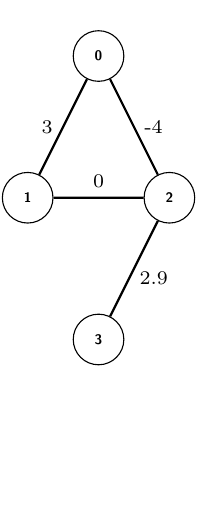
\begin{tikzpicture}[scale=1.8,auto,swap]
                    \node[vertex] (0) at (0.5,3) {0};
                    \node[vertex] (1) at (0,2) {1};
                    \node[vertex] (2) at (1,2) {2};
                    \node[vertex] (3) at (0.5,1) {3};

                    \path[edge] (0) -- node[weight,left] {3} (1);
                    \path[edge] (0) -- node[weight,right] {-4} (2);
                    \path[edge] (1) -- node[weight,above] {0} (2);
                    \path[edge] (2) -- node[weight,right,pos=0.6] {2.9} (3);

                    \pgfresetboundingbox
                    \path [use as bounding box] (0,0) rectangle (1,3.2);
                \end{tikzpicture}
            \end{figure}
        \end{column}%
    \end{columns}
\end{frame}

\begin{frame}[plain]{Minimum spanning tree}
    \begin{itemize}
        \item We have an undirected weighted graph
        \item The vertices along with a subset of the edges in the graph is called a spanning tree if
            \begin{itemize}
                \item it forms a tree (i.e.\ does not contain a cycle) and
                \item the tree spans all vertices (all vertices can reach all other vertices)
            \end{itemize}
        \vspace{10pt}
        \item The weight of a spanning tree is the sum of the weights of the edges in the subset
        \vspace{10pt}
        \item We want to find a minimum spannig tree
    \end{itemize}
\end{frame}

\begin{frame}[plain]{Minimum spanning tree}
    \begin{itemize}
        \item Several greedy algorithms work
        \vspace{10pt}
        \item Go through the edges in the graph in increasing order of weight
        \item Greedily pick an edge if it doesn't form a cycle (Union-Find can be used to keep track of when we would get a cycle)
        \item When we've gone through all edges, we have a minimum spanning tree
        \vspace{10pt}
        \item This is Kruskal's algorithm
        \item Time complexity is $O(E \log E)$
        \item Other algorithms are Prim's and Boruvska's
    \end{itemize}
\end{frame}

\begin{frame}[plain,fragile]{Minimum spanning tree}
    \begin{minted}[fontsize=\scriptsize]{cpp}

bool edge_cmp(const edge &a, const edge &b) {
    return a.weight < b.weight;
}

vector<edge> mst(int n, vector<edge> edges) {
    union_find uf(n);
    sort(edges.begin(), edges.end(), edge_cmp);

    vector<edge> res;
    for (int i = 0; i < edges.size(); i++) {
        int u = edges[i].u,
            v = edges[i].v;

        if (uf.find(u) != uf.find(v)) {
            uf.unite(u, v);
            res.push_back(edges[i]);
        }
    }

    return res;
}
    \end{minted}
\end{frame}

\begin{frame}[plain]{Shortest paths}
    \begin{itemize}
        \item We have a weighted graph (undirected or directed)
        \item Given two vertices $u,v$, what is the shortest path from $u$ to $v$?
        \vspace{10pt}
        \item If all weights are the same, this can be solved with breadth-first search
        \item Of course, this is usually not the case...
    \end{itemize}
\end{frame}

\begin{frame}[plain]{Shortest paths}
    \begin{itemize}
        \item There are many known algorithms to find shortest paths
        \item Like breadth-first search, these algorithms usually find the shortest paths from a given start vertex to all other vertices
        \vspace{5pt}
        \item Let's take a quick look at Dijkstra's algorithm, the Bellman-Ford algorithm and the Floyd-Warshall algorithm
    \end{itemize}
\end{frame}

\begin{frame}[plain,fragile]{Dijkstra's algorithm}
    \tiny
    \begin{minted}{cpp}
vector<edge> adj[100];
vector<int> dist(100, INF);

void dijkstra(int start) {
    dist[start] = 0;
    priority_queue<pair<int, int>,
                   vector<pair<int, int> >,
                   greater<pair<int, int> > > pq;
    pq.push(make_pair(dist[start], start));

    while (!pq.empty()) {
        int u = pq.top().second;
        pq.pop();

        for (int i = 0; i < adj[u].size(); i++) {
            int v = adj[u][i].v;
            int w = adj[u][i].weight;

            if (w + dist[u] < dist[v]) {
                dist[v] = w + dist[u];
                pq.push(make_pair(dist[v], v));
            }
        }
    }
}
    \end{minted}
\end{frame}

\begin{frame}[plain]{Dijkstra's algorithm}
    \begin{itemize}
        \item Time complexity is $O(V \log E)$
        \vspace{10pt}
        \item Note that this only works for non-negative weights
    \end{itemize}
\end{frame}

\begin{frame}[plain,fragile]{Bellman-Ford algorithm}
    \begin{minted}[fontsize=\footnotesize]{cpp}
vector<edge> adj[100];
vector<int> dist(100, INF);

void bellman_ford(int n, int start) {

    dist[start] = 0;

    for (int i = 0; i < n - 1; i++) {
        for (int u = 0; u < n; u++) {
            for (int j = 0; j < adj[u].size(); j++) {
                int v = adj[u][j].v;
                int w = adj[u][j].weight;
                dist[v] = min(dist[v], w + dist[u]);
            }
        }
    }
}
    \end{minted}
\end{frame}

\begin{frame}[plain]{Bellman-Ford algorithm}
    \begin{itemize}
        \item Time complexity is $O(V\times E)$
        \vspace{10pt}
        \item Can be used to detect negative-weight cycles, how?
        \item <2-> At most $N$ edges in a path before it contains a cycle.
        \item <3-> Do extra iterations on the outer loop.
        \item <4-> If there is any change then there is at least one negative weight cycle.
    \end{itemize}
\end{frame}

\begin{frame}[plain]{Floyd-Warshall algorithm}
    \begin{itemize}
        \item What about using dynamic programming to compute shortest paths?
        \vspace{10pt}
    \item Let $\mathrm{sp}(k, i, j)$ be the shortest path from $i$ to $j$ if we're only allowed to travel through the vertices $0$, \ldots, $k$
        \vspace{5pt}
    \item Base case: $\mathrm{sp}(k, i, j) = 0$ if $i = j$
    \item Base case: $\mathrm{sp}(-1, i, j) = \mathrm{weight}[i][j]$ if $(i,j) \in E$
    \item Base case: $\mathrm{sp}(-1, i, j) = \infty$
        \vspace{5pt}
    \item $\mathrm{sp}(k, i, j) = \mathrm{min} \left\{
	\begin{array}{l}
        \mathrm{sp}(k - 1, i, k) + \mathrm{sp}(k - 1, k, j) \\
        \mathrm{sp}(k - 1, i, j)
	\end{array}
\right.$
    \end{itemize}
\end{frame}

\begin{frame}[plain,fragile]{Floyd-Warshall algorithm}
    \begin{minted}[fontsize=\scriptsize]{cpp}
int dist[1000][1000];
int weight[1000][1000];

void floyd_warshall(int n) {
    for (int i = 0; i < n; i++) {
        for (int j = 0; j < n; j++) {
            dist[i][j] = i == j ? 0 : weight[i][j];
        }
    }

    for (int k = 0; k < n; k++) {
        for (int i = 0; i < n; i++) {
            for (int j = 0; j < n; j++) {
                dist[i][j] = min(dist[i][j], dist[i][k] + dist[k][j]);
            }
        }
    }
}
    \end{minted}
\end{frame}

\begin{frame}[plain]{Floyd-Warshall algorithm}
    \begin{itemize}
\item Computes all-pairs shortest paths
\item Time complexity is clearly $O(n^3)$
\item Very simple to code
    \end{itemize}
\end{frame}

\begin{frame}[plain,fragile]{Floyd-Warshall algorithm}
    \begin{minted}[fontsize=\scriptsize]{cpp}
int dist[1000][1000];
int weight[1000][1000];

void floyd_warshall(int n) {
    rep(i,0,n) rep(j,0,n)
        dist[i][j] = i == j ? 0 : weight[i][j];

    rep(k,0,n) rep(i,0,n) rep(j,0,n)
        dist[i][j] = min(dist[i][j], dist[i][k] + dist[k][j]);
}
    \end{minted}
\end{frame}

\end{document}
